\begin{figure*}[t]
    \centering
    \IfFileExists{figures/gdsq_pipeline.png}{%
        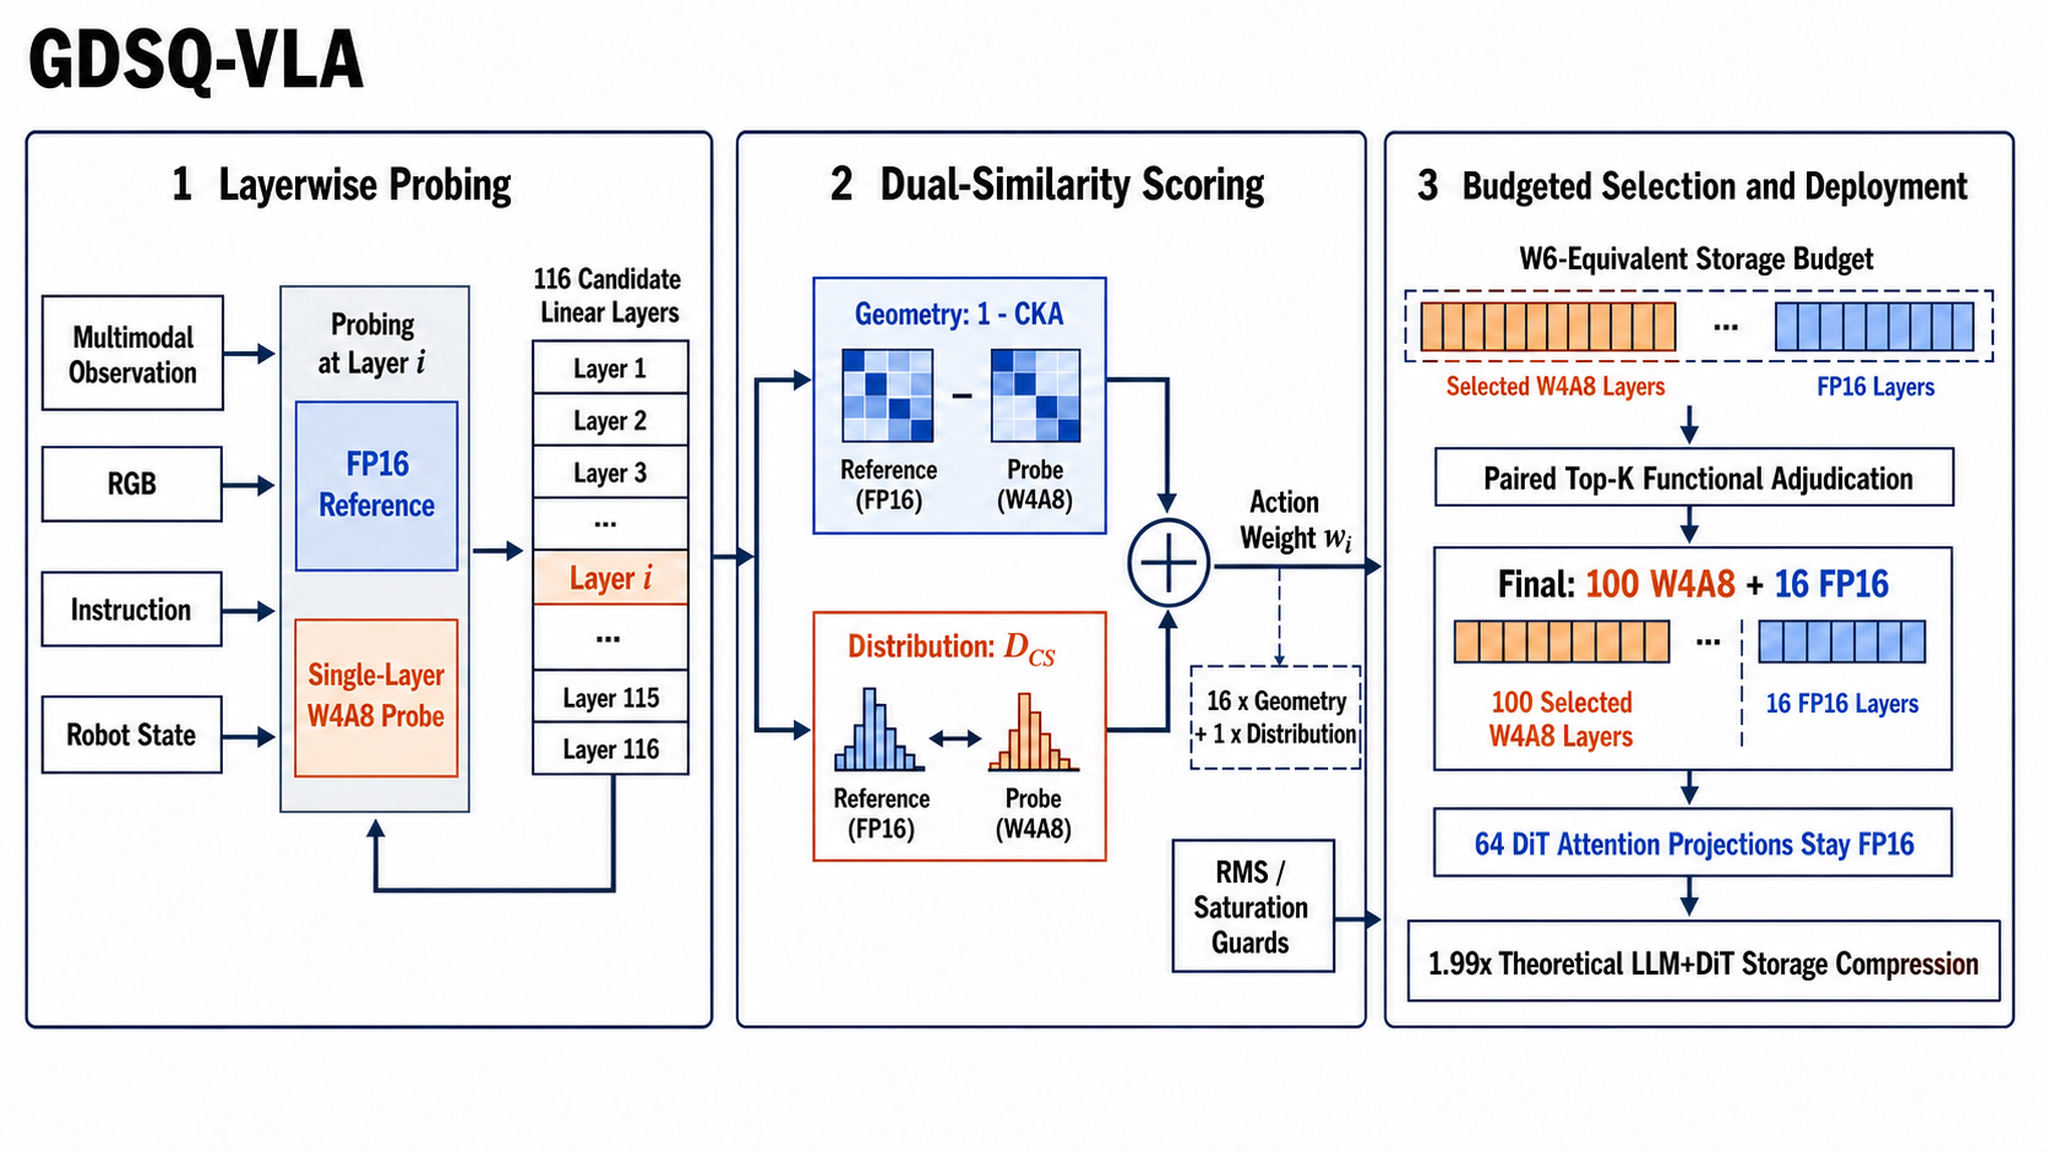
\includegraphics[width=\textwidth]{figures/gdsq_pipeline.png}%
    }{%
        \setlength{\fboxsep}{7pt}%
        \fbox{%
        \begin{minipage}{0.96\textwidth}
        \centering
        \textbf{GPT-Image 2 figure placeholder -- final prompt is included in the source tree}\\[5pt]
        \begin{tabular}{>{\centering\arraybackslash}p{0.28\textwidth}
                        >{\centering\arraybackslash}p{0.30\textwidth}
                        >{\centering\arraybackslash}p{0.30\textwidth}}
        \textbf{1. Layerwise Probing} & \textbf{2. Dual-Similarity Scoring} & \textbf{3. Selection and Deployment} \\
        RGB + instruction + state & $16(1-\mathrm{CKA}) + D_{\mathrm{CS}}$ & W6-equivalent storage budget \\
        FP16 reference vs. one-layer W4A8 & action weight + hard guards & Top-$K$ functional adjudication \\
        116 candidate Linear layers & geometry + distribution & 100 W4A8 + 16 FP16
        \end{tabular}
        \end{minipage}}
    }
    \caption{Overview of \method. A single-layer intervention protocol measures complementary geometric and distributional representation changes, weights them by action-level sensitivity, and applies hard feasibility guards. A budgeted selector proposes diverse W4/FP16 masks, which are adjudicated by paired action-generation behavior before freezing the final 16:1 configuration. The 64 DiT attention projections outside the 116-layer candidate set remain in FP16.}
    \label{fig:pipeline}
\end{figure*}
